\documentclass[12pt, oneside, openany]{article}
\usepackage[T1]{fontenc}
\usepackage[spanish, es-tabla, es-lcroman]{babel}
\usepackage[utf8]{inputenc}
\usepackage[document]{ragged2e}
\usepackage{tcolorbox}
\tcbuselibrary{theorems}
\usepackage{cancel}
\usepackage{amssymb}
\usepackage{amsmath}
\usepackage{mathrsfs}
\usepackage{wrapfig}
\usepackage{fancyhdr}
\usepackage{colortbl}
\usepackage{longtable}
\usepackage{graphicx}
\usepackage{subcaption}
\usepackage{xcolor}
\usepackage{tikz}
\usetikzlibrary{positioning}
\usepackage{multicol}
\usepackage{multirow}
\usepackage{lastpage}
\usepackage{pdfpages}
\usepackage{listings}
\usepackage{blindtext}
\spanishdecimal{.}
\usepackage[explicit]{titlesec}
\usepackage[colorlinks=true, linkcolor=black, citecolor=black, urlcolor=blue]{hyperref}
\usepackage[a4paper, total={16cm, 24cm}]{geometry}
\pagestyle{fancy}
\lhead{Muñoz Nuñez Ian Emmanuel}
\rhead{Proyecto 6}
\lfoot{Mtra. María Patricia Ventura Nuñez}
\rfoot{CUCEI}
\renewcommand{\headrulewidth}{1pt}
\renewcommand{\footrulewidth}{1pt}

\setlength{\headheight}{14.49998pt}

\begin{document}

\begin{titlepage}
    \pagenumbering{roman}
    \centering
    {\bfseries\LARGE Universidad de Guadalajara \par}
    \vfill
    {
        \includegraphics[width=0.3\linewidth]{UdG.png}
        \includegraphics[width=0.3\linewidth]{qci.png}
        \par
    }
    \vfill
    {\bfseries\LARGE Seminario de problemas de programación de sistemas reconfigurables \par}
    \vfill
    {\LARGE Diseño e implementación de varias funciones combinacionales utilizando páginas diferentes en una memoria \emph{EEPROM} \par}
    \vfill
    {\bfseries\LARGE Nombre: \par}
    \vfill
    {\bfseries\LARGE Muñoz Nuñez Ian Emmanuel \par}
    \vfill
    {\bfseries\LARGE Sección: D01 \par}
    \vfill
    {\bfseries\LARGE Código: 216464457 \par}
    \vfill
    {\bfseries\LARGE Maestra: \par}
    \vfill
    {\bfseries\LARGE María Patricia Ventura Nuñez \par}
    \vfill
    {\bfseries\LARGE Ingeniería robótica \par}
\end{titlepage}

\pagenumbering{arabic}
\newpage

\section{Objetivo}
{\sffamily\large
    \hspace{0.5cm} Solucionar problemas de diseño utilizando las herramientas aprendidas en programación de sistemas reconfigurables.
    
    \hspace{0.5cm} Utilizar hojas de datos de las familias lógicas.
    
    \hspace{0.5cm} Simular circuitos digitales en programas de diseño como \emph{Proteus\texttrademark} e implementarlos físicamente.
    
    \hspace{0.5cm} Diseño e implementación de varias funciones combinacionales utilizando páginas diferentes en una memoria \emph{EPROM} o \emph{EEPROM}. Ejemplo:
    
    \renewcommand{\labelitemi}{$\bullet$}
    \begin{itemize}
        \item Operaciones aritméticas.
        \item Código de estudiante.
        \item Nombre.
        \item Carrera.
    \end{itemize}
    
}

\section{Material}
{\sffamily\large
    \renewcommand{\labelitemi}{$\bullet$}
    \begin{itemize}
        \item Protoboard.
        \item Fuente VCC (5V).
        \item Resistencias de 200$\Omega$ y 2k$\Omega$.
        \item Dip switch de 8 bits.
        \item Display de 7 segmentos.
        \item Memoria \emph{EEPROM 24C64B}.
    \end{itemize}
    
}

\newpage
\section{Marco teórico}
\subsection{Tabla de verdad para la página 3 (300) - Multiplicador}
{\sffamily\large
    \begin{table}[h!]
        \centering
        \sffamily
        \scalebox{1.25}{
        \begin{tabular}{|c||c|c|c|c||c|c|c|c||c|c|c|c||c||c|}
            \hline
              &  &  &  &  & p & g & f & e & d & c & b & a & Hexadecimal & \\
            \hline
            0 &  0 & 0 & 0 & 0 &  0 & 0 & 1 & 1 & 1 & 1 & 1 & 1 &  3F & 0 \\
            \hline
            1 &  0 & 0 & 0 & 1 &  0 & 0 & 1 & 1 & 1 & 1 & 1 & 1 &  3F & 0 \\
            \hline
            2 &  0 & 0 & 1 & 0 &  0 & 0 & 1 & 1 & 1 & 1 & 1 & 1 &  3F & 0 \\
            \hline
            3 &  0 & 0 & 1 & 1 &  0 & 0 & 1 & 1 & 1 & 1 & 1 & 1 &  3F & 0 \\
            \hline
            4 &  0 & 1 & 0 & 0 &  0 & 0 & 1 & 1 & 1 & 1 & 1 & 1 &  3F & 0 \\
            \hline
            5 &  0 & 1 & 0 & 1 &  0 & 0 & 0 & 0 & 0 & 1 & 1 & 0 &  06 & 1 \\
            \hline
            6 &  0 & 1 & 1 & 0 &  0 & 1 & 0 & 1 & 1 & 0 & 1 & 1 &  5B & 2 \\
            \hline
            7 &  0 & 1 & 1 & 1 &  0 & 1 & 0 & 0 & 1 & 1 & 1 & 1 &  4F & 3 \\
            \hline
            8 &  1 & 0 & 0 & 0 &  0 & 0 & 1 & 1 & 1 & 1 & 1 & 1 &  3F & 0 \\
            \hline
            9 &  1 & 0 & 0 & 1 &  0 & 1 & 0 & 1 & 1 & 0 & 1 & 1 &  5B & 2 \\
            \hline
            A &  1 & 0 & 1 & 0 &  0 & 1 & 1 & 0 & 0 & 1 & 1 & 0 &  66 & 4 \\
            \hline
            B &  1 & 0 & 1 & 1 &  0 & 1 & 1 & 1 & 1 & 1 & 0 & 1 &  7D & 6 \\
            \hline
            C &  1 & 1 & 0 & 0 &  0 & 0 & 1 & 1 & 1 & 1 & 1 & 1 &  3F & 0 \\
            \hline
            D &  1 & 1 & 0 & 1 &  0 & 1 & 0 & 0 & 1 & 1 & 1 & 1 &  4F & 3 \\
            \hline
            E &  1 & 1 & 1 & 0 &  0 & 1 & 1 & 1 & 1 & 1 & 0 & 1 &  7D & 6 \\
            \hline
            F &  1 & 1 & 1 & 1 &  0 & 1 & 1 & 0 & 0 & 1 & 1 & 1 &  67 & 9 \\
            \hline
        \end{tabular}
        }
        \caption{\sffamily Tabla de verdad para la página 3}
        \label{tab:verdad3}
    \end{table}
    
}

\newpage
\subsection{Tabla de verdad para la página 6 (600) - Nombre}
{\sffamily\large
    \begin{table}[h!]
        \centering
        \sffamily
        \scalebox{1.25}{
        \begin{tabular}{|c||c|c|c|c||c|c|c|c||c|c|c|c||c||c|}
            \hline
             &  &  &  &  &  p & g & f & e & d & c & b & a & Hexadecimal & \\
            \hline
            0 &  0 & 0 & 0 & 0 &  0 & 0 & 0 & 0 & 0 & 1 & 1 & 0 &  06 & I \\
            \hline
            1 &  0 & 0 & 0 & 1 &  0 & 1 & 1 & 1 & 0 & 1 & 1 & 1 &  77 & A \\
            \hline
            2 &  0 & 0 & 1 & 0 &  0 & 1 & 0 & 1 & 0 & 1 & 0 & 0 &  54 & n \\
            \hline
            3 &  0 & 0 & 1 & 1 &  0 & 1 & 1 & 1 & 1 & 0 & 0 & 1 &  79 & E \\
            \hline
            4 &  0 & 1 & 0 & 0 &  0 & 1 & 0 & 0 & 1 & 1 & 1 & 1 &  4F & 3 \\
            \hline
            5 &  0 & 1 & 0 & 1 &  0 & 1 & 1 & 1 & 0 & 1 & 1 & 1 &  77 & A \\
            \hline
            6 &  0 & 1 & 1 & 0 &  0 & 1 & 0 & 0 & 1 & 1 & 1 & 1 &  4F & 3 \\
            \hline
            7 &  0 & 1 & 1 & 1 &  0 & 0 & 1 & 1 & 1 & 1 & 1 & 0 &  3E & U \\
            \hline
            8 &  1 & 0 & 0 & 0 &  0 & 1 & 0 & 1 & 0 & 1 & 0 & 1 &  55 & ñ \\
            \hline
            9 &  1 & 0 & 0 & 1 &  0 & 0 & 1 & 1 & 1 & 1 & 1 & 1 &  3F & O \\
            \hline
            A &  1 & 0 & 1 & 0 &  0 & 1 & 0 & 1 & 1 & 0 & 1 & 1 &  5B & 2 \\
            \hline
            B &  1 & 0 & 1 & 1 &  0 & 1 & 0 & 1 & 0 & 1 & 0 & 0 &  54 & n \\
            \hline
            C &  1 & 1 & 0 & 0 &  0 & 0 & 1 & 1 & 1 & 1 & 1 & 0 &  3E & U \\
            \hline
            D &  1 & 1 & 0 & 1 &  0 & 1 & 0 & 1 & 0 & 1 & 0 & 1 &  55 & ñ \\
            \hline
            E &  1 & 1 & 1 & 0 &  0 & 1 & 1 & 1 & 1 & 0 & 0 & 1 &  79 & E \\
            \hline
            F &  1 & 1 & 1 & 1 &  0 & 1 & 0 & 1 & 1 & 0 & 1 & 1 &  5B & 2 \\
            \hline
        \end{tabular}
        }
        \caption{\sffamily Tabla de verdad para la página 6}
        \label{tab:verdad6}
    \end{table}
    
}

\newpage
\subsection{Tabla de verdad para la página 9 (900) - Carrera}
{\sffamily\large
    \begin{table}[h!]
        \centering
        \sffamily
        \scalebox{1.25}{
        \begin{tabular}{|c||c|c|c|c||c|c|c|c||c|c|c|c||c||c|}
            \hline
             &  &  &  &  & p & g & f & e & d & c & b & a & Hexadecimal & \\
             \hline
             0 &  0 & 0 & 0 & 0 &  0 & 0 & 0 & 0 & 0 & 1 & 1 & 0 &  06 & I \\
             \hline
             1 &  0 & 0 & 0 & 1 &  0 & 1 & 0 & 1 & 0 & 1 & 0 & 0 &  54 & n \\
             \hline
             2 &  0 & 0 & 1 & 0 &  0 & 1 & 1 & 0 & 1 & 1 & 1 & 1 &  6F & g \\
             \hline
             3 &  0 & 0 & 1 & 1 &  1 & 0 & 0 & 0 & 0 & 0 & 0 & 0 &  80 & . \\
             \hline
             4 &  0 & 1 & 0 & 0 &  0 & 1 & 0 & 1 & 0 & 0 & 0 & 0 &  50 & r \\
             \hline
             5 &  0 & 1 & 0 & 1 &  0 & 0 & 1 & 1 & 1 & 1 & 1 & 1 &  3F & O \\
             \hline
             6 &  0 & 1 & 1 & 0 &  0 & 1 & 1 & 1 & 1 & 1 & 0 & 0 &  7C & b \\
             \hline
             7 &  0 & 1 & 1 & 1 &  0 & 0 & 1 & 1 & 1 & 1 & 1 & 1 &  3F & O \\
             \hline
             8 &  1 & 0 & 0 & 0 &  0 & 1 & 1 & 1 & 1 & 0 & 0 & 0 &  78 & t \\
             \hline
             9 &  1 & 0 & 0 & 1 &  0 & 0 & 0 & 0 & 0 & 1 & 1 & 0 &  06 & I \\
             \hline
             A &  1 & 0 & 1 & 0 &  0 & 0 & 1 & 1 & 1 & 0 & 0 & 1 &  39 & C \\
             \hline
             B &  1 & 0 & 1 & 1 &  0 & 1 & 1 & 1 & 0 & 1 & 1 & 1 &  77 & A \\
             \hline
             C &  1 & 1 & 0 & 0 &  0 & 1 & 1 & 1 & 0 & 1 & 1 & 0 &  76 & H \\
             \hline
             D &  1 & 1 & 0 & 1 &  0 & 0 & 1 & 1 & 1 & 1 & 1 & 1 &  3F & O \\
             \hline
             E &  1 & 1 & 1 & 0 &  0 & 0 & 1 & 1 & 1 & 0 & 0 & 0 &  38 & L \\
             \hline
             F &  1 & 1 & 1 & 1 &  1 & 1 & 1 & 1 & 0 & 1 & 1 & 1 &  F7 & A \\
             \hline
        \end{tabular}
        }
        \caption{\sffamily Tabla de verdad para la página 9}
        \label{tab:verdad9}
    \end{table}
    
}

\newpage
\subsection{Tabla de verdad para la página 12 (c00) - Código}
{\sffamily\large
    \begin{table}[h!]
        \centering
        \sffamily
        \scalebox{1.25}{
        \begin{tabular}{|c||c|c|c|c||c|c|c|c||c|c|c|c||c||c|}
            \hline
             &  &  &  &  & p & g & f & e & d & c & b & a & Hexadecimal & \\
            \hline
            0 &  0 & 0 & 0 & 0 &  0 & 1 & 0 & 1 & 1 & 0 & 1 & 1 &  5B & 2 \\
            \hline
            1 &  0 & 0 & 0 & 1 &  0 & 0 & 0 & 0 & 0 & 1 & 1 & 0 &  06 & 1 \\
            \hline
            2 &  0 & 0 & 1 & 0 &  0 & 1 & 1 & 1 & 1 & 1 & 0 & 1 &  7D & 6 \\
            \hline
            3 &  0 & 0 & 1 & 1 &  0 & 1 & 1 & 0 & 0 & 1 & 1 & 0 &  66 & 4 \\
            \hline
            4 &  0 & 1 & 0 & 0 &  0 & 1 & 1 & 1 & 1 & 1 & 0 & 1 &  7D & 6 \\
            \hline
            5 &  0 & 1 & 0 & 1 &  0 & 1 & 1 & 0 & 0 & 1 & 1 & 0 &  66 & 4 \\
            \hline
            6 &  0 & 1 & 1 & 0 &  0 & 1 & 1 & 0 & 0 & 1 & 1 & 0 &  66 & 4 \\
            \hline
            7 &  0 & 1 & 1 & 1 &  0 & 1 & 1 & 0 & 1 & 1 & 0 & 1 &  6D & 5 \\
            \hline
            8 &  1 & 0 & 0 & 0 &  0 & 0 & 0 & 0 & 0 & 1 & 1 & 1 &  07 & 7 \\
            \hline
            9 &  1 & 0 & 0 & 1 &  0 & 1 & 1 & 0 & 0 & 1 & 1 & 1 &  67 & 9 \\
            \hline
            A &  1 & 0 & 1 & 0 &  0 & 1 & 1 & 1 & 1 & 1 & 1 & 1 &  7F & 8 \\
            \hline
            B &  1 & 0 & 1 & 1 &  0 & 1 & 1 & 0 & 0 & 1 & 1 & 1 &  67 & 9 \\
            \hline
            C &  1 & 1 & 0 & 0 &  0 & 1 & 1 & 0 & 1 & 1 & 0 & 1 &  6D & 5 \\
            \hline
            D &  1 & 1 & 0 & 1 &  0 & 1 & 0 & 1 & 1 & 1 & 1 & 0 &  5E & d \\
            \hline
            E &  1 & 1 & 1 & 0 &  0 & 0 & 1 & 1 & 1 & 1 & 1 & 1 &  3F & 0 \\
            \hline
            F &  1 & 1 & 1 & 1 &  0 & 0 & 0 & 0 & 0 & 1 & 1 & 0 &  06 & 1 \\
            \hline
        \end{tabular}
        }
        \caption{\sffamily Tabla de verdad para la página 12}
        \label{tab:verdad12}
    \end{table}
    
}

\newpage
\section{Procedimiento}
{\sffamily\large
    \hspace{0.5cm} Primero se obtuvo la tabla de verdad para cada una de las páginas de la memoria. Una vez teniendo las salidas deseadas, se convirtieron a \emph{hexadecimal} para programar la memoria.
    
    \hspace{0.5cm} Realizar el circuito de este proyecto en proto fue sencillo, el único problema fueron las conexiones de la memoria, pues al principio pensé que algunas entradas o salidas estaban mal, o que había un error en la programación de la memoria, pero solo había que conectar las entradas que no se usaban a \emph{tierra} para que la memoria las tomara como si estuvieran negadas.
    
    \hspace{0.5cm} Los materiales utilizados son: 1 dip switch de 8 bits, 8 resistencias de 2k$\Omega$ y 8 de 220$\Omega$, un display de 7 segmentos de cátodo común y una memoria \emph{EEPROM 28C64B}.
    
}

\section{Circuito a implementar}
\subsection{Simulación}
{\sffamily\large
    \hspace{0.5cm} En la siguiente página se muestra el diseño del circuito en simulación.
}

\newpage
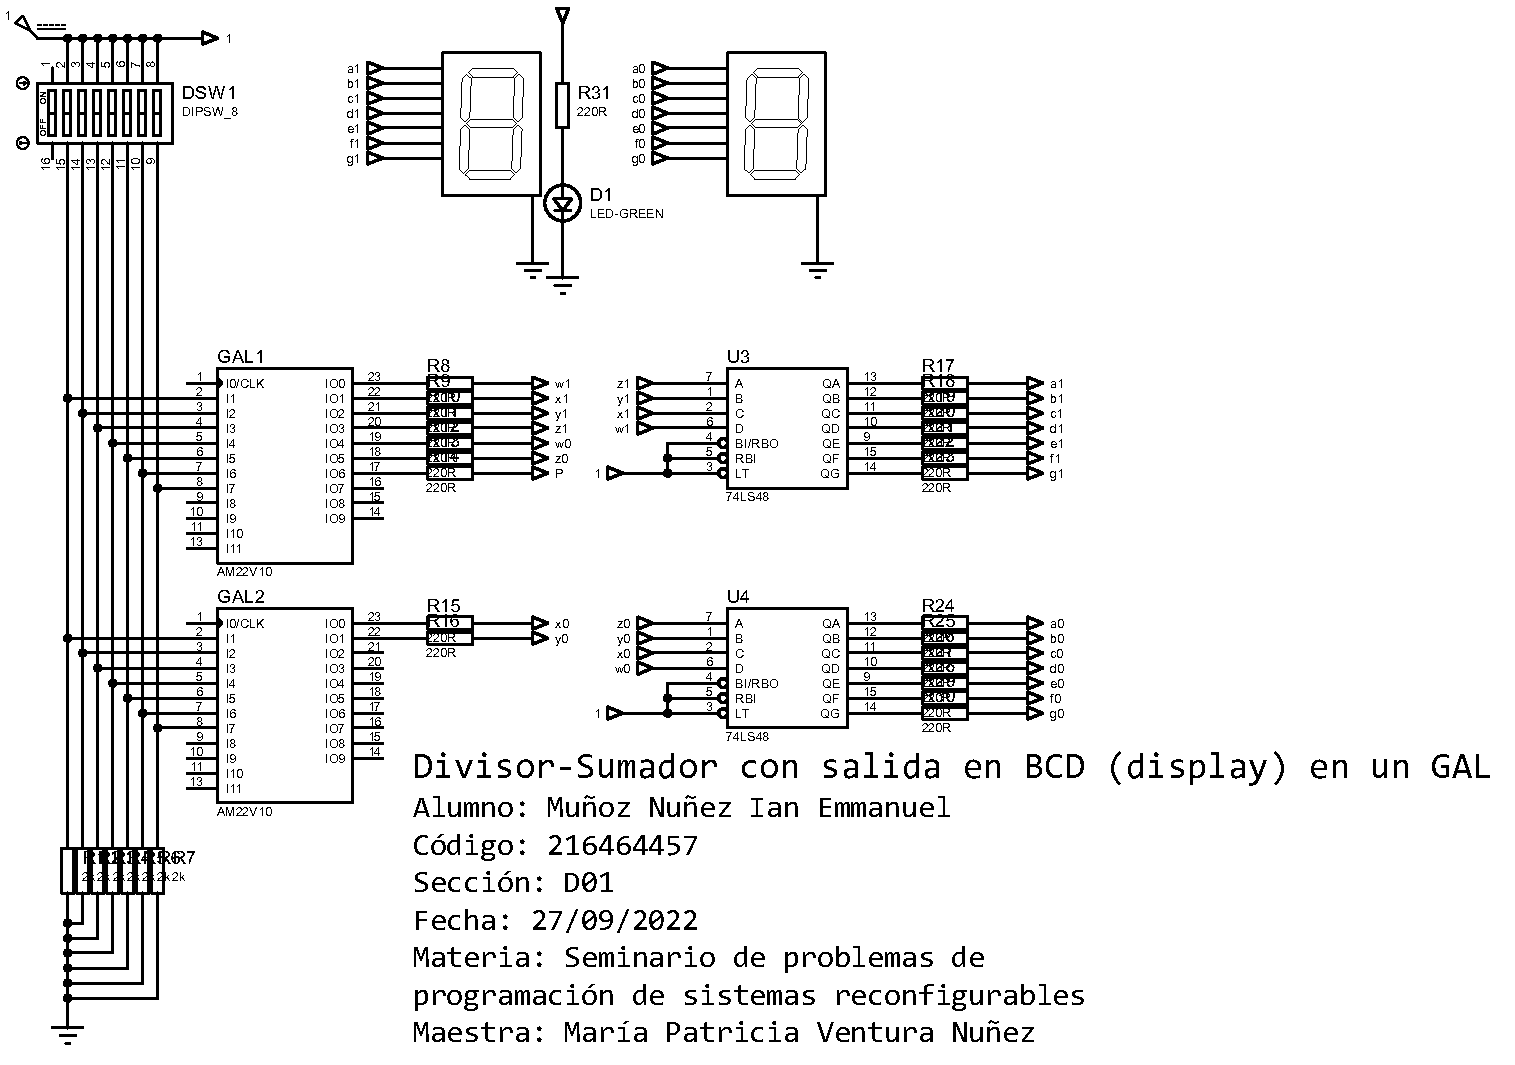
\includepdf[pages={1}]{main.PDF}

\newpage
\subsection{Protoboard}
\begin{figure}[h!]
    \centering
    
    \begin{subfigure}[tl]{0.45\textwidth}
        \centering
        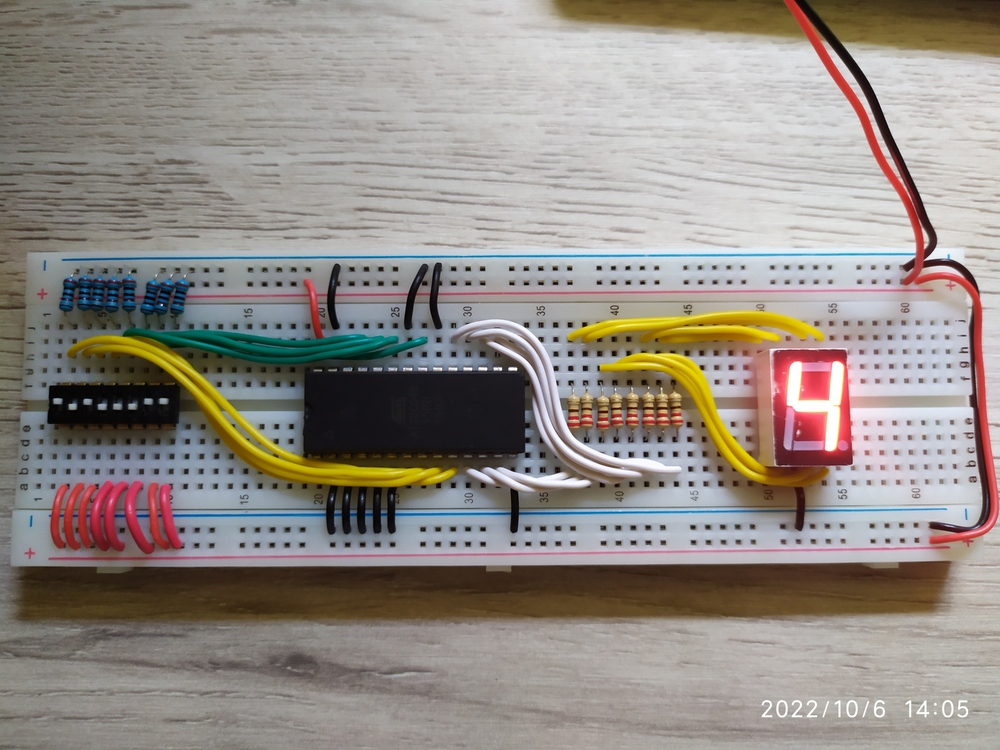
\includegraphics[width=\linewidth]{IMG_20221006_140505.jpg}
    \end{subfigure}
    \begin{subfigure}[tr]{0.45\textwidth}
        \centering
        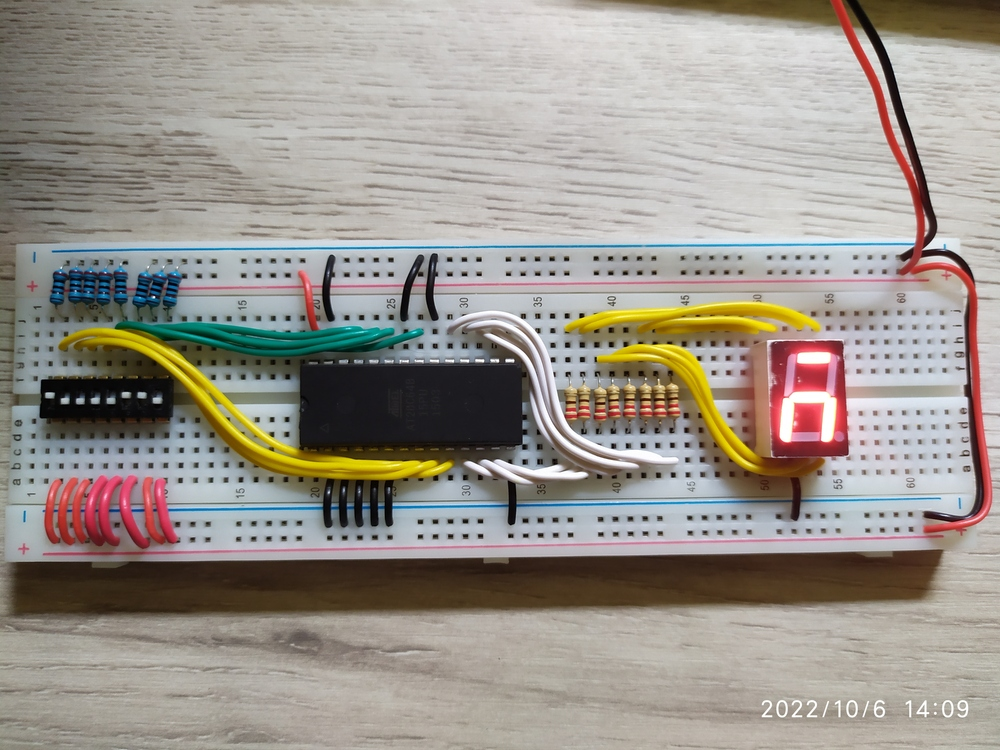
\includegraphics[width=\linewidth]{IMG_20221006_140909.jpg}
    \end{subfigure}
    \begin{subfigure}[bl]{0.45\textwidth}
        \centering
        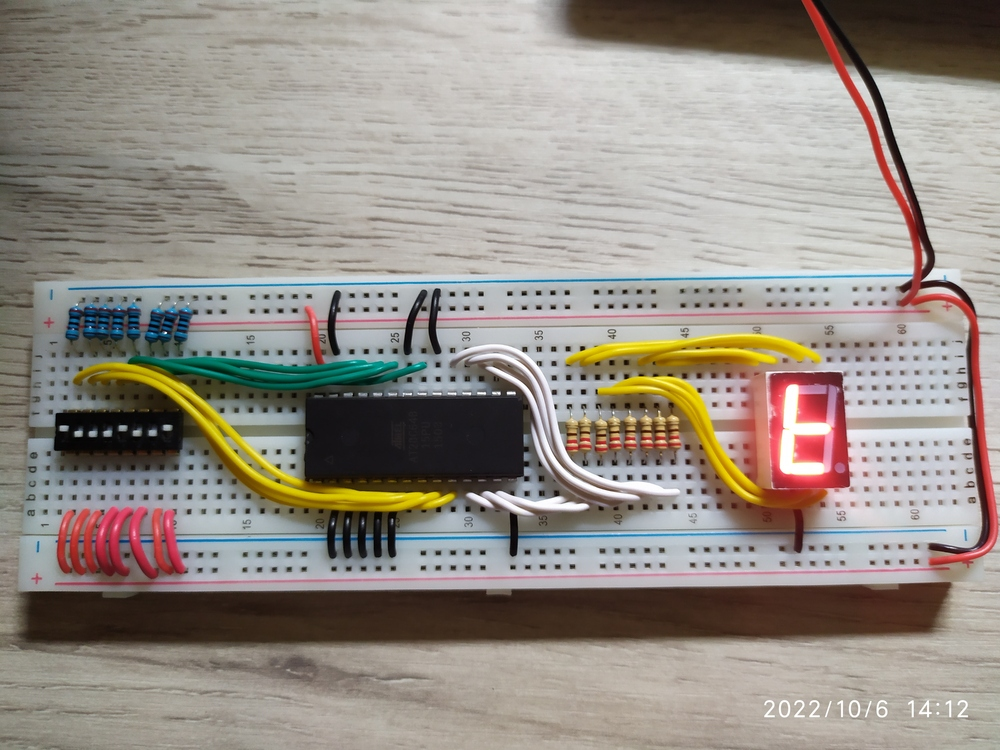
\includegraphics[width=\linewidth]{IMG_20221006_141226.jpg}
    \end{subfigure}
    \begin{subfigure}[br]{0.45\textwidth}
        \centering
        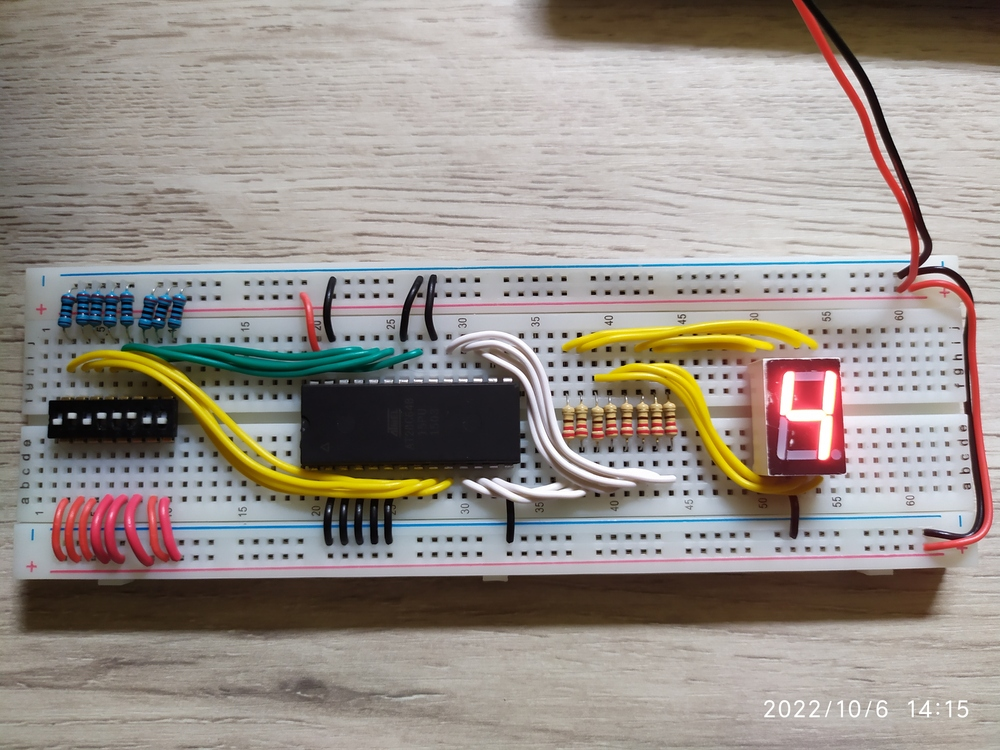
\includegraphics[width=\linewidth]{IMG_20221006_141505.jpg}
    \end{subfigure}
    
    \caption{\sffamily Circuito en protoboard}
    \label{fig:proto}
\end{figure}

\section{Conclusión}
{\sffamily\large
    \hspace{0.5cm} Este proyecto fue más interesante y sencillo que el anterior, pues, además del problema que tuve con las conexiones de la memoria, lo más complicado fue hacer las tablas de verdad de cada página. Prefiero usar la \emph{EEPROM} a la \emph{GAL}, pues creo que fue más sencilla de programar y usar.
}

\end{document}
